\subsection{Data Analysis Plan}

After the flight the collected samples, from the CAC and the AAC, will be analyzed with a Picarro G2401 gas analyzer. The end of the CAC tube that remains closed during sampling will be opened first and connected to the gas standard with the higher CO$_2$ and CH$_4$ concentrations. This is to have a notable difference between the standard gas and the stratospheric air sample. The other end of the CAC tube will be connected to the analyzer. The analyzer pump will pull the sample through the analyzer with both ends of the CAC open. The sample that entered the AirCore last, will go into the analyzer first, and will represent the beginning of the concentration time trace, while the lowest sampled pressure followed by the standard gas, will flag the end of the AirCore sample time trace. After the sample finish, the standard gas will be pulled through the analyzer, \cite{Karion}, \cite{Olivier}.
After the sample has been analyzed, the time trace of analysis will be converted into a mole fraction profile as a function of atmospheric pressure, using the ideal gas law,
\begin{equation}
    PV = nRT <=> n = \frac{PV}{RT}
    \label{eq:idealgaslaw}
\end{equation}
where P is the ambient pressure, V is the inner volume of the CAC/AAC, n the fraction of moles, R is the universal gas constant in $J K^{-1} mol^{-1}$ and T the ambient temperature in Kelvin, \cite{Olivier}. 
A constant unit of pressure in the atmosphere is represented by a unit of length in the CAC tube, due to the method that the CAC will sample the ambient air.
During the analysis the number of moles that will go through the analyzer will increase linearly with time. So, the number of moles at any time during the analysis will be
\begin{equation}
    n_i = n^{max}\frac{t_i}{\Delta t}
    \label{eq:ni}
\end{equation}
where $n^{max}$ is the maximum number of moles i.e when the CAC reaches the Earth's surface, and $\Delta t$ is the total time duration of the analysis between the top and bottom of the CAC sample.   
Finally, the vertical profiles will be obtained by using equations \ref{eq:idealgaslaw} and \ref{eq:ni}, and relate a specific pressure point with every Picarro measurement of the sample.   

The AAC sampling system will be analyzed, in the same manner as the CAC, using the same Picarro gas analyzer. After the recovery of the AAC, and considering that the picarro analyzer shows stable readings of the calibrating gas, one bag at a time will be connected to the analyzer. The readings of the analyzer, will be corresponding to calibration gas, bag's sample, and calibration gas again. The sample of the bag will be known since its concentration will be different then that of the concentration of the standard gas. As such, changes gas concentration readings will indicate that the air from the sample bag is being analyzed. Corrections should be possible, for both AAC and CAC. Since the calibration's gas concentrations are already known, they are going to be compared with the analyzer's reading and corrected if necessary. For the CAC and AAC, the values will be interpolated with the actual concentrations of the calibration gas and the corrected sample will be obtained. The vertical profiles for CO$_2$ and CH$_4$ are going to be obtained using again, equations \ref{eq:idealgaslaw} and \ref{eq:ni}. 


\subsubsection{Picarro G2401}

The analyzer that will be used is the model Picarro G2401. It uses near-infrared Cavity Ring Down Spectroscopy technology and is capable of measuring four atmospheric trace gases simultaneously and continuously ($CO, CO_2, CH_4, H_2O$).\\
The CRDS technique's basic principle is shown in Figure \ref{fig:CRDS}. Light from a semiconductor diode laser is used. There is an optical cavity filled with the gas that has to be analyzed and the aim is to determine the decay time of the diode laser light. As it can be seen in Figure \ref{fig:CRDS}, the sample gas is introduced in a cavity with 3 high-reflectivity mirrors. When the laser is shut off, the light that was circulating in the cavity decays with a characteristic time which is measured. If the wavelength of the injected light does not match any absorption feature of any gas in the cavity, the decay time is dominated by mirror loss and it is very long. On the other side, when the wavelength of the injected light is resonant with an absorption feature of a species in the cavity, the decay time is short and decreases as the reciprocal of the species concentration.



\begin{figure}[H]
    \begin{align*}
        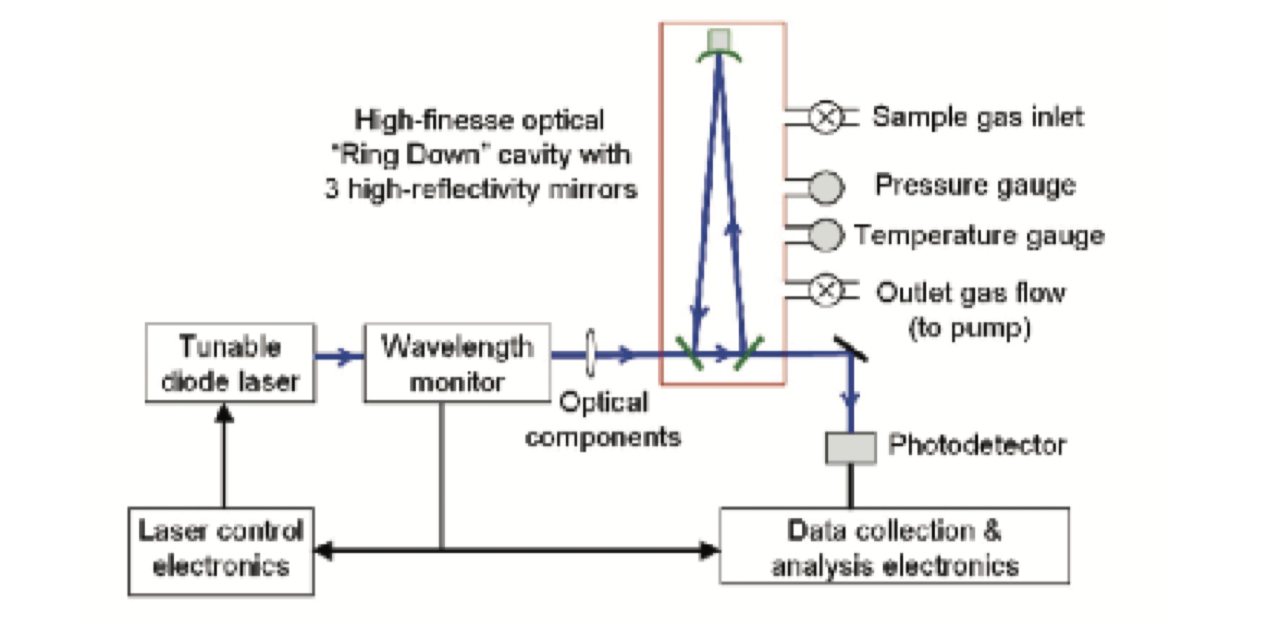
\includegraphics[width=0.9\linewidth]{7-data-analysis-and-results/img/CRDS.png}
    \end{align*}
    \caption{Schematics of CRDS analyzer showing optical cavity and sample gas flow. \cite{Picarro}\label{fig:CRDS}}
\end{figure}


Figure \ref{fig:Picarro-interfaces} shows the back of the analyzer with gas supply, electrical and computer connections. The analyzer can be configured to deliver data in different formats: digital or analogue. When the main power is turned on the analyzer will automatically start, including the Graphical User Interface (GUI). 

\begin{figure}[H]
    \begin{align*}
        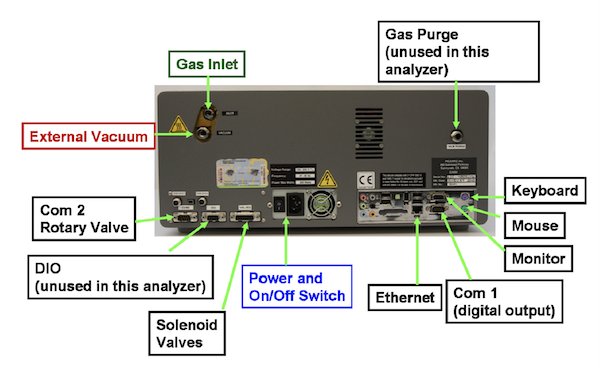
\includegraphics[width=0.9\linewidth]{7-data-analysis-and-results/img/Picarro-interfaces.png}
    \end{align*}
    \caption{Back of Picarro G2401 analyzer showing gas supply, electrical and computer connections. \cite{Picarrouserguide}\label{fig:Picarro-interfaces}}
\end{figure}